\def\projectfigsize{5}
\begin{figure}
{\centering
    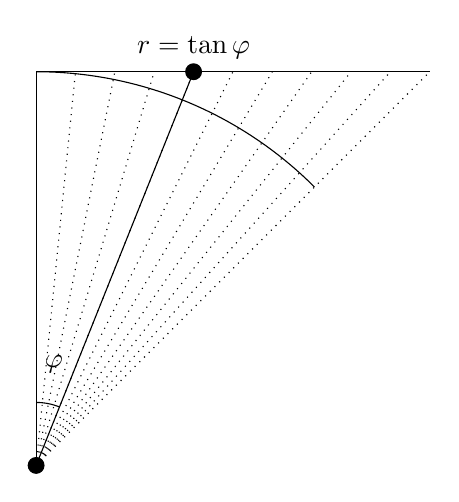
\begin{tikzpicture}
        \draw (45:\projectfigsize) arc (45:90:\projectfigsize);
        \draw (0,\projectfigsize) -- (\projectfigsize,\projectfigsize);
        \filldraw (0,0) circle (.1);
        \filldraw (2,5) circle (.1);
        \foreach \x in {0,0.5,...,\projectfigsize}
            \draw[dotted] (0,0) -- (\x,\projectfigsize);
        \draw (0,0) -- (0,\projectfigsize); 
        \draw (0,0) -- (2,\projectfigsize);
        \draw (90:.8) arc (90:68.19:.8);
        \path +(80:1.3) node {$\varphi$};
        \path +(2,5.3) node {$r=\tan \varphi$};
    \end{tikzpicture}
    \includegraphics[width=0.5\textwidth]{gnomonic.png}
    \caption[Gnomonic projection]{The gnomonic projection maps dip direction (longtitude of normal vector) and dip (colatitude of normal vector) into polar coordinates $r$ and $\theta$. Left: A cross-section along a single line of longtitude $\theta$ is displayed. ($\theta$ does not change during the projection so no new variable is introduced.) Right: Great-circles are mapped to straight lines because a) all great circles are coplanar with the sphere's center, and b) any two non-parallel planes intersect at a line~\parencite{marozols_gnomonic_2022}.}
    \label{gnomonic}
}
\end{figure}